\section{Árboles y Grafos en Computación}

Un árbol es una clase especial de grafo y su importancia es tal en las aplicaciones computacionales que lo estudiaremos en una sección por separado.
Junto con el estudio de árboles surge el de problemas de optimización sobre grafos que también tocaremos en esta sección.

\subsection{Árboles}

Supongamos que tenemos una red de computadores como la de la figura~\ref{fig:network} donde los trazos entre computadores representan cables directos entre ellos.
\begin{figure}[h!]
\centering
\includegraphics[width=400pt]{eps_imgs/network}
\caption{Una red de computadores.}
\label{fig:network}
\end{figure}
Esta red cumple con la propiedad de que cualquier computador puede enviar información a cualquier otro en la red (no necesariamente en forma directa), o sea, el grafo asociado a la red es conexo.
Supongamos que quisiéramos construir una red con la propiedad anterior (todos los computadores se puedan comunicar entre ellos) pero minimizando la cantidad de conexiones directas entre computadores.
Un posible resultado se ve en la figura~\ref{fig:tree-network}.
\begin{figure}[h!]
\centering
\includegraphics[width=400pt]{eps_imgs/tree-network}
\caption{Una red de computadores con el mínimo número de conexiones directas.}
\label{fig:tree-network}
\end{figure}
Esta red cumple la misma propiedad anterior, todo computador puede enviar información a cualquier otro computador en la red.
Si nos enfocamos en el grafo asociado a esta nueva red de computadores, una característica crucial que lo diferencia con el anterior es que dado cualquier par de vértices (computadores en la red) existe un único camino que los une.
A un grafo con estas características se le llama {\bf árbol} y su definición se formaliza a continuación.

\begin{definicion}
Un grafo $T=(V(T),E(T))$ es un {\bf árbol} si para cada par de vértices $u,v\in V(T)$ existe un único camino de $u$ a $v$.
Es inmediato de la definición que un árbol es siempre un grafo conexo, dado que para cada par de vértices \emph{existe} un camino (que ``de paso'' es único).
\end{definicion}

\begin{ejemplo}
El grafo correspondiente a la red de la figura~\ref{fig:tree-network} es un árbol.
El grafo de la figura~\ref{fig:graph25} también es un árbol, para comprobarlo basta con notar que entre cualquier par de vértices existe un único camino.
\begin{figure}[h!]
\centering
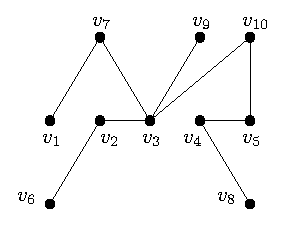
\includegraphics{eps_imgs/graph25}
\caption{Un árbol.}
\label{fig:graph25}
\end{figure}
\end{ejemplo}

En computación generalmente usamos una clase particular de árboles en los que un vértice particular se distingue de los demás, a este vértice se le llama {\bf raíz} del árbol.

\begin{definicion}
Un {\bf árbol con raíz} (o árbol enraizado, \emph{rooted tree} en inglés) es un árbol $T=(V(T),E(T))$ en que uno de sus vértices $r\in V(T)$ se ha distinguido de los demás. 
Al vértice distinguido $r$ se le llama {\bf raíz} del árbol.
Los vértices en un árbol (con o sin raíz) que tienen grado igual a 1 se llaman {\bf hojas}
(también consideraremos hoja a un vértice de grado 0).
Definiremos más conceptos más adelante.
\end{definicion}
Cuando dibujemos un árbol con raíz, el vértice correspondiente a la raíz se dibujará siempre ``arriba'' y los vértices hoja se dibujarán ``abajo''.
El nombre de árbol se ve motivado por el resultado de dibujar un grafo de estas características, como se puede ver en la figura~\ref{fig:tree}.
\begin{figure}[h!]
\centering
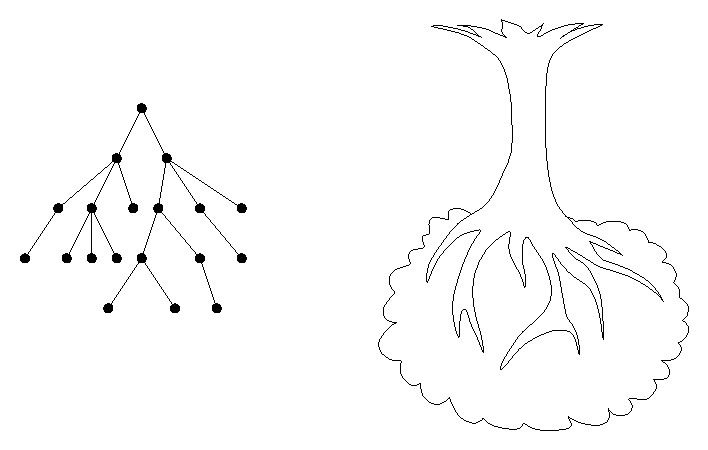
\includegraphics{eps_imgs/tree}
\caption{Árboles (izquierda) en computación y (derecha) en el mundo real... bueno, casi.}
\label{fig:tree}
\end{figure}

Los siguientes teoremas nos entregan caracterizaciones de árboles, formas alternativas de definirlos.

\begin{teorema}
Un grafo $T$ es un árbol si y sólo si $T$ es conexo y no tiene ciclos.\footnote{Aquí nos referimos claramente a ciclos compuestos por más de un único vértice, o sea, a ciclos de largo mayor a 0.}

\begin{demostracion}
$(\Rightarrow)$ Primero si $T$ es un árbol es por definición conexo, nos falta demostrar entonces que un árbol no puede tener ciclos.
Supongamos que $T$ tuviese un ciclo, y sea $C$ un ciclo en $T$ que pasa por los vértices $u$ y $v$.
Supongamos que $C$ parte (y termina) en $u$, entonces $C$ es de la forma $(u,\ldots,v,\ldots,u)$, por lo que se puede dividir en dos porciones, una para ir de $u$ a $v$, digamos $p_1$, y otra (distinta ya que un ciclo no repite aristas) para ir de $v$ a $u$, digamos $p_2$.
Resulta entonces que $p_1$ y $p_2$ son dos caminos distintos entre $u$ y $v$ en $T$, lo que contradice el hecho de que $T$ es un árbol.
La figura~\ref{fig:no-cycle} muestra un diagrama del anterior argumento.
Finalmente $T$ no puede tener ciclos.
\begin{figure}[h!]
\centering
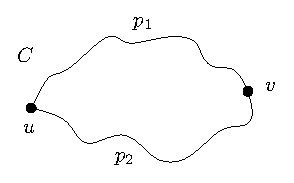
\includegraphics{eps_imgs/no-cycle}
\caption{Formación de dos caminos distintos entre $u$ y $v$ a partir de un ciclo que los contiene.}
\label{fig:no-cycle}
\end{figure}

$(\Leftarrow)$ Como $T$ es conexo, para cada par de vértices existe un camino que los une, falta demostrar que ese camino es único.
Supongamos entonces que $T$ no tiene ciclos pero que sin embargo existe un par de vértices con dos caminos distintos uniéndolos en $T$.
Sea $u$ y $v$ estos vértices y sean $p_1$ y $p_2$ los dos caminos distintos en $T$ que unen a $u$ con $v$.
Dado que estos caminos son distintos entonces ambos tienen al menos tres vértices.
Sea $x$ el vértice anterior al primer vértice que diferencia a $p_1$ y $p_2$ (note que $x_1$ está en $p_1$ y en $p_2$).
Sea $y$ el vértice siguiente a $x$ que pertenece simultáneamente a $p_1$ y $p_2$.
Un diagrama de esto se ve en la figura~\ref{fig:no-two-paths}.
\begin{figure}[h!]
\centering
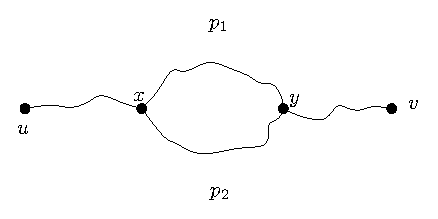
\includegraphics{eps_imgs/no-two-paths}
\caption{Dos caminos distintos entre el mismo par de vértices siempre contienen un ciclo.}
\label{fig:no-two-paths}
\end{figure}
El camino entre $x$ e $y$ a través de $p_1$ junto con el camino entre $x$ e $y$ a través de $p_2$ forman un ciclo en $T$ lo que contradice nuestra hipótesis de que $T$ no tiene ciclos.
Finalmente no pueden existir dos caminos distintos entre $u$ y $v$, de donde concluimos que para todo par de vértices en $T$ existe un único camino que los une y por lo tanto $T$ es un árbol.
\end{demostracion}
\end{teorema}

\begin{corolario}
Un grafo $T$ es un árbol si y sólo si todas sus aristas son de corte, o sea, para cualquier arista $e$ el grafo $T-e$ no es conexo.

\begin{demostracion}\label{teo:cut-tree}
$(\Rightarrow)$ En la sección anterior (teorema~\ref{teo:cut-edge}) demostramos que una arista es de corte si y sólo si no pertenece a ningún ciclo en el grafo.
Ahora, $T$ es un árbol si y sólo si $T$ es conexo y no tiene ningún ciclo, si y sólo si todas sus aristas cumplen con la propiedad de no pertenecer a un ciclo, si y sólo si, todas sus aristas son de corte.
\end{demostracion}
\end{corolario}

Este corolario debió ser evidente, dado que un árbol tiene el mínimo número de aristas necesarias para que el grafo sea conexo, el sacar cualquier arista desconecta al grafo.
El siguiente corolario no es tan evidente.

\begin{corolario}
Todo árbol es un grafo bipartito.

\begin{demostracion}
En la sección anterior (teorema~\ref{teo:odd-cycle}) demostramos que un grafo es bipartito si y sólo si no contiene ciclos de largo impar.
Si $T$ es un árbol $T$ no contiene ningún ciclo y por lo tanto $T$ es bipartito.
\end{demostracion}
\end{corolario}

La siguiente es una propiedad muy simple de los árboles lo que nos permitirá hacer demostraciones por inducción sobre ellos.

\begin{lema}
Sea $T$ un árbol y $v$ una hoja de $T$, entonces el grafo $T-v$ es también un árbol.

\begin{demostracion}
Para demostrar que el grafo $T-v$ es un árbol debemos comprobar que para cualquier par de vértices en $T-v$, existe un único camino que los une.
Sea $u$ y $w$ dos vértices en $T$ distintos de $v$, y sea la secuencia $P=(u,u_1,u_2,\ldots,u_n,w)$ el único camino en $T$ que une a $u$ con $w$. 
Es claro que el vértice $v$ no aparece en $P$ ya que todos los vértices de $P$ (excepto $u$ y $w$) deben tener grado al menos 2, luego si eliminamos $v$ de $T$ no afecta al camino entre $u$ y $w$, luego el camino $P=(u,u_1,u_2,\ldots,u_n,w)$ entre $u$ y $w$ en $T-v$.
Como la demostración la hicimos en general para un par de vértices cualquiera, en $T-v$ existe un único camino entre todo par de vértices y por lo tanto $T-v$ también es un árbol.
\end{demostracion}
\end{lema}

Con el anterior lema podemos demostrar el siguiente teorema que es una caracterización muy simple de un árbol

\begin{teorema}\label{teo:tree-edges}
Un grafo $T$ con $n$ vértices es un árbol si y sólo si es conexo y tiene exactamente $n-1$ aristas.

\begin{demostracion}
$(\Rightarrow)$ Si $T$ es un árbol con $n$ vértices, entonces claramente es conexo, falta demostrar que tiene exactamente $n-1$ aristas, lo haremos por inducción en $n$.
\begin{inducciondemo}
  \BI Si $n=1$ tenemos un árbol con sólo un vértice y sin aristas, por lo que se cumple la propiedad (la cantidad de aristas es igual a $0 = 1-1 = n-1$).
  \HI Supongamos que un árbol con $n$ vértices tiene exactamente $n-1$ aristas.
  \TI Sea ahora $T$ un árbol con $n+1$ vértices, queremos demostrar que $T$ tiene exactamente $(n+1)-1=n$ aristas.
  Centrémonos en una hoja $v$ cualquiera de este árbol.
  Por el lema anterior $T-v$ también es un árbol y tiene exactamente $n$ vértices por lo que se aplica la HI, luego $T-v$ tiene exactamente $n-1$ aristas.
  Dado que $v$ es una hoja, $v$ tiene grado 1 en $T$ y por lo tanto $T$ tiene exactamente una arista más que $T-v$, o sea $T$ tiene exactamente $n$ aristas, por lo que se cumple la propiedad.
\end{inducciondemo}
Por inducción simple se sigue que todo árbol con $n$ vértices tiene exactamente $n-1$ aristas.

$(\Leftarrow)$ En la sección anterior demostramos  en el teorema~\ref{teo:min-components} que un grafo con $n$ vértices y $k$ aristas tiene al menos $n-k$ componentes conexas.
Si $T$ es un grafo conexo con $n$ vértices y exactamente $n-1$ aristas y tomamos una arista $e$ cualquiera de $T$, entonces dado que $T-e$ tiene $n-2$ aristas, por el teorema~\ref{teo:min-components}, $T-e$ tiene al menos dos componentes conexas y por lo tanto $e$ es una arista de corte.
Dado que elegimos $e$ como una arista cualquiera, $T$ cumple con que todas sus aristas son de corte y por lo tanto (corolario~\ref{teo:cut-tree}) $T$ es un árbol.

\end{demostracion}
\end{teorema}

En nuestro ejemplo inicial nos preguntábamos por la mínima cantidad de conexiones directas necesarias para hacer una red de computadores de manera tal que cualquier computador pudiera enviar información a cualquier otro en la red.
Dado que esto se logra cuando el grafo asociado a la red es un árbol, el teorema anterior nos dice que si tenemos $n$ computadores, la mínima cantidad de estas conexiones será $n-1$.
Este teorema nos da también una forma rápida de chequear si un grafo conexo es o no un árbol, sólo debemos verificar que tenga exactamente una arista menos que vértices.

\subsection{Árboles en Computación}

Ya mencionamos que en computación generalmente usamos árboles con raíz.
Esta noción motiva varias otras definiciones sobre árboles en aplicaciones computacionales.

\begin{definicion}
Sea $T=(V(T),E(T))$ un árbol con raíz $r$, note que, dado que $T$ es un árbol, para cada vértice $x\in V(T)$ existe un único camino de $r$ a $x$.
Definimos lo siguiente:
\begin{itemize}
  \itemsep 0pt
  \item El largo del único camino entre $r$ y un vértice cualquiera $x$ se llama {\bf profundidad} de $x$.
  La raíz $r$ tiene profundidad $0$.
  \item El máximo de las profundidades de todos los vértices de $T$ se llama {\bf altura del árbol} (o {\bf profundidad del árbol}).
  \item La {\bf altura} de un vértice $x$ es la altura del árbol menos la profundidad de $x$.
  \item El conjunto de vértices que aparecen en el único camino de $r$ a $x$ se llaman {\bf ancestros} de $x$.
  Note que $x$ es un ancestro de sí mismo.
  A veces usaremos el término ancestros propios de $x$  para referirnos a los ancestros de $x$ distintos de $x$.
  \item El ancestro propio de $x$ de mayor profundidad se llama {\bf padre} de $x$. 
  Un vértice $x$ es {\bf hijo} de su padre.
  Note que $r$ no tiene padre y que los vértices hoja no tienen hijos.
  \item Si dos vértices $x$ e $y$ tienen el mismo padre diremos que $x$ e $y$ son {\bf hermanos}.
\end{itemize}
La figura~\ref{fig:tree-concepts} muestra gráficamente estas definiciones.

\begin{figure}[h!]
\centering
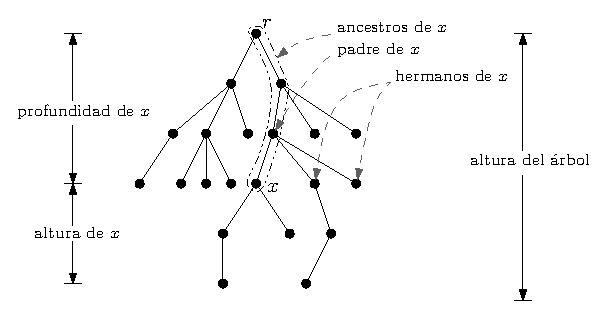
\includegraphics[height=170pt]{eps_imgs/tree-concepts}
\caption{Definiciones sobre un árbol}
\label{fig:tree-concepts}
\end{figure}
\end{definicion}

Muchas aplicaciones de ordenamiento y búsqueda en computación usan estructuras de datos basadas en un tipo especial de árboles, los llamado árboles binarios.

\begin{definicion}
Un árbol con raíz se dice {\bf árbol binario} si todo vértice tiene a lo más grado 3, o equivalentemente (y cómo se usa más comunmente en computación), si todo vértice tiene a lo más 2 hijos.
En un árbol binario, los hijos de un vértice particular se distinguen en {\bf hijo izquierdo} e {\bf hijo derecho}, lo que también normará las posiciones en las que se dibujen los hijos de cierto vértice.

Note que si a un árbol binario se le elimina una hoja, el grafo que resulta es también un árbol binario (la demostración se deja como ejercicio).
\end{definicion}

Estudiaremos algunas propiedades de los árboles binarios y veremos un caso particular muy útil de este tipo de árboles.

\begin{teorema}
La cantidad de hojas de un árbol binario es uno más la cantidad de vértices con exactamente dos hijo.

\begin{demostracion}
Usaremos la propiedad descrita con anterioridad acerca de que un árbol binario al que se le saca una hoja sigue siendo binario, con esto haremos una demostración por inducción en la cantidad de vértices del árbol binario.
\begin{inducciondemo}
  \BI El caso base es un árbol compuesto por sólo un vértice, la raíz.
  Un árbol de estas características tiene sólo una hoja y ningún vértice con dos hijos, luego cumple la propiedad.
  \HI Supongamos que un árbol binario con $n$ vértices tiene una hoja más que vértices con dos hijos.
  \TI Sea $T$ un árbol binario con $n+1$ vértices, queremos demostrar que $T$ tiene una hoja más que vértices con dos hijos.
  Sea $v$ una hoja cualquiera de $T$, sabemos que $T-v$ es también un árbol binario y tiene exactamente $n$ vértices (uno menos que $T$) por lo que $T-v$ cumple con HI, o sea tiene una hoja más que vértices con dos hijos.
  Supongamos que $T-v$ tiene $k$ vértices con dos hijos entonces por HI tiene $k+1$ hojas >qué podemos decir de $T$?
  Lo que podamos decir dependerá de si $v$ (la hoja que le sacamos) tenía o no un hermano.
  \begin{itemize}
    \item[-] Si $v$ tiene un hermano en $T$, entonces el padre de $v$ es un vértice con dos hijos en $T$.
    Ahora, en el árbol $T-v$, el vértice que era padre de $v$ tiene sólo un hijo.
    Lo anterior quiere decir que $T$ tiene exactamente un vértice más con dos hijos que $T-v$, o sea que $T$ tiene exactamente $k+1$ vértices con dos hijos.
    Ahora también ocurre que $T$ tiene exactamente una hoja más que $T-v$, o sea que $T$ tiene $k+2$ hojas.
    Hemos concluido que $T$ tiene $k+2$ hojas y $k+1$ vértices con dos hijos y por lo tanto cumple con la propiedad.
    \item[-] Si $v$ no tiene hermano, entonces el vértice padre de $v$ en $T$ se convierte en una hoja en el árbol $T-v$, lo que quiere decir que $T$ y $T-v$ tienen exactamente la misma cantidad de hojas, $k+1$.
    El único vértice que ve afectado su cantidad de hijos en $T-v$ es el padre de $v$, este tiene exactamente un hijo en $T$ y $0$ hijos en $T-v$ por lo que la cantidad de vértices con dos hijos en $T$ es también la misma que en $T-v$ e igual a $k$.
    Hemos concluido que $T$ tiene $k+1$ hojas y $k$ vértices con dos hijos y por lo tanto cumple con la propiedad.
  \end{itemize}
  Por inducción en la cantidad de vértices se sigue que todo árbol binario tiene exactamente una hoja más que vértices con dos hijos.
\end{inducciondemo}
\end{demostracion}
\end{teorema}

\begin{ejemplo}
  Un torneo de eliminación simple es un torneo en que cada competencia se realiza entre dos participantes, el participante que pierde la competencia se va del torneo.
  El último participante que permanece en el torneo es el ganador.
  Un ejemplo típico de un torneo de eliminación simple es un campeonato de tenis.
  
  Un torneo de eliminación simple se puede representar por un árbol binario, los participantes iniciales corresponden a las hojas del árbol, el padre de dos vértices corresponde al participante ganador en la competencia realizada entre sus dos hijos, y el participante representado por la raíz del árbol corresponde al ganador del torneo.
   Los ``niveles'' del árbol, o sea las distintas alturas de los vértices, representan las ``rondas'' del torneo, y vértices hojas que no se encuentre a altura $0$ corresponden a participantes que pasan ``libre'' algunas rondas (esto suele ocurrir por ejemplo en los torneos de tenis).
   En la figura~\ref{fig:world-cup-tournament} se ve el resultado de un ``hipotético'' campeonato mundial de futbol desde los cuartos de final, representado por un árbol binario.
   En la figura~\ref{fig:tournament} se ve un torneo más general con participantes que pasan libres ciertas rondas.
   
   \begin{figure}[t!]
   \centering
   \vspace*{200pt}
   %\includegraphics{eps_imgs/world-cup-tournament}
   \caption{Cuartos de final del campeonato mundial de futbol.}
   \label{fig:world-cup-tournament}
   \end{figure}
   \begin{figure}[h!]
   \centering
   \vspace*{200pt}
   %\includegraphics{eps_imgs/tournament}
   \caption{Un torneo de eliminación simple en general con participantes libres en ciertas rondas.}
   \label{fig:tournament}
   \end{figure}
   
   Queremos responder la siguiente pregunta, si tenemos $n$ participantes en un torneo de eliminación simple >cuántos partidos (competencias entre dos participantes) en total se deberán realizar durante el torneo?
   Se podría pensar que esto dependerá de la organización particular del torneo, sin embargo, si nos fijamos que cualquier torneo se puede representar por un árbol binario podremos responder esta pregunta independiente de las decisiones de la organización.
   Ya hemos dicho que cada hoja del árbol asociado corresponde a un participante inicial en el torneo.
   Si un vértice del árbol tiene dos hijos, este corresponde al ganador de un partido entre sus dos vértices hijos, por lo que podríamos asociar un partido con cada vértice que tiene dos hijos en el árbol.
   Finalmente, el teorema anterior nos dice que si el un árbol hay $n$ hojas, entonces la cantidad de vértices con dos hijos es exactamente $n-1$, luego $n-1$ será la cantidad de partidos necesaria realizar durante el campeonato.
   Por ejemplo, $100$ participantes del torneo darán lugar a $99$ partidos en total.
\end{ejemplo}

Una clase especial de árboles binarios nos ayudan para establecer casos límites y cotas para algunos algoritmos de búsqueda, estos son los árboles binarios completos que definiremos a continuación.

\begin{definicion}
  Diremos que $T$ es un {\bf árbol binario completo} si es un árbol binario que cumple con que todos sus vértices que no son hoja tienen exactamente dos hijos y que todas las hojas se encuentran a la misma profundidad.
  
  Si $T$ es un árbol (no necesariamente binario completo) y $v$ es un vértice cualquiera de $T$, el {\bf sub-árbol con raíz en $v$} será el sub-grafo de $T$ compuesto por $v$, todos los vértices que tienen a $x$ como ancestros, y todas las aristas que conectan a estos vértices.
  Es claro que un sub-árbol es también un árbol, que un sub-árbol de un árbol binario es también un árbol binario, y que un sub-árbol de un árbol binario completo es también un árbol binario completo.
\end{definicion}

\begin{teorema}
Un árbol binario completo de altura $H$ tiene exactamente $2^H$ hojas

\begin{demostracion} Por inducción en la altura del árbol
\end{demostracion}
\end{teorema}

\begin{corolario}
Un árbol binario completo de altura $H$ tiene exactamente $2^{H+1}-1$ vértices.

\begin{demostracion}
$2^H$ hojas $\Rightarrow$ $2^{H}-1$ vértices con dos hijos $\rightarrow$ $2^H+2^{H}-1=2^{H+1}-1$ vértices en total.
\end{demostracion}
\end{corolario}

\begin{corolario}
En un árbol binario completo con $n$ vértices su altura es menor o igual que $\log_2(n)$.

\begin{demostracion}
Si la altura es $H$, claramente $n\geq 2^H\Rightarrow \log_2(n)\geq H$.
\end{demostracion}
\end{corolario}

\subsection{Grafos en Computación}
Generalmente en computación nos interesa resolver problemas de optimización sobre grafos para esto el modelo de grafos se extiende un poco.
Las siguientes definiciones introducen el tema.

\begin{definicion}
Un {\bf grafo con peso} es una estructura $G=(V(G),E(G),w)$ donde $V(G)$ es un conjunto de vértices, $E(G)$ es un conjunto de aristas (tal como en un grafo normal) y $w$ es una función de \emph{peso} (o \emph{costo}) $w:E(G)\rightarrow\N$ que a cada arista $e$ de $G$ le asigna un valor que llamaremos peso $w(e)$ (a veces la función puede tener otro conjutno de llegada como $\Z$ o incluso $\R$).
Cuando dibujamos un grafo con peso, generalmente etiquetamos cada arista con su peso correspondiente.

El peso o costo de un camino (caminata, ciclo) en un grafo con peso, es la sumatoria de los pesos de las aristas que componen el camino (caminata, ciclo).
Cuando queremos representar un grafo con peso usando una matriz, usamos una matriz en que cada posición tiene el peso de la arista correspondiente, $0$'s en la diagonal, e $\infty$ si la arista correspondiente no existe (representando que la arista existe pero su peso es demasiado alto como para ser tomada en cuenta).
\end{definicion}

En la figura~\ref{fig:graph26} se muestra un ejemplo de grafo con peso cuya matriz asociada es:
\begin{figure}
\centering
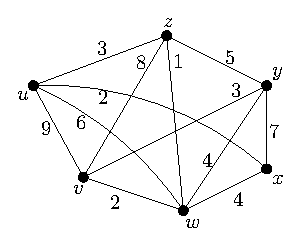
\includegraphics{eps_imgs/graph26}
\caption{Ejemplo de un grafo con peso.}
\label{fig:graph26}
\end{figure}
\[
\left[
\begin{array}{cccccc}
0 & 9 & 6 & 2 & \infty & 3 \\
9 & 0 & 2 & \infty & 3 & 8 \\
6 & 2 & 0 & 4 & 4 & 1 \\
2 & \infty & 4 & 0 & 7 & \infty \\
\infty & 3 & 4 & 7 & 0 & 5 \\
3 & 8 & 1 &\infty & 5 & 0 \\
\end{array}\right]
\]
Sobre un grafo como este se pueden hacer muchas preguntas de optimización como por ejemplo cuál es el camino de menor peso total entre un par de vértices.
En la figura para los vértices $u$ y $v$, la respuesta es $(u,z,w,v)$ de peso total $6$.
El anterior problema suele llamarse el problema del camino más corto.
Cuando estudiamos árboles los introducimos como el grafo con menos aristas que mantiene la propiedad de ser conexo, nos podríamos preguntar en este contexto cuál es el árbol asociado al grafo que tiene menor peso total (siendo el peso total del árbol la suma de los pesos de todas las aristas).
En el grafo de la figura el árbol es el compuesto por las aristas $zw$, $ux$, $vw$, $uz$, $vy$.
El anterior problema suele llamarse el problema del árbol de cobertura de costo mínimo.
Para los dos problemas anteriores existen métodos eficientes que los resuelven, estos métodos suelen estudiarse en detalle en un curso de Algoritmos y Estructuras de Datos.
Otra pregunta que puede hacerse es acerca del ciclo Hamiltoniano de peso total mínimo, sin embargo nuevamente ocurre que para este problema no existe un algoritmo eficiente.

Existen otros tipos de grafos que se usan generalmente para problemas de búsqueda.

\begin{definicion}
Un {\bf grafo dirigido} es una estructura $G=(V(G),E(G))$ muy similar a un grafo normal, pero en que la relación ``ser vecino de'' no necesariamente es simétrica, de echo en un gafo dirigido el conjunto $E(G)$ es un conjunto de pares ordenados de vértices, $E(G)\subseteq V(G)\times V(G)$.

Las definiciones de camino y ciclo se extienden a {\bf camino dirigido} y {\bf ciclo dirigido}.
\end{definicion}

En un grafo normal (no dirigido) estudiamos el problema de la componente conexa.
En un grafo dirigido podemos estudiar un problema similar, cuál conjunto de vértices cumplen la propiedad de que entre cada par de ellos existe un camino dirigido.
Este es el problema de encontrar las componentes {\bf fuertemente conexas} de un grafo.

Se pueden hacer modelos que combinen las dos definiciones anteriores, grafos dirigidos con peso. 
En el se pueden plantear problemas como el de camino dirigido más corto, flujos máximos (suponiendo que el peso de una arista dirigida es la capacidad de un canal), etc.

[...falta completar...]

